%||||---------------
\begin{frame}
  \frametitle{Cyclus Modular Architecture and Open Development}
  The combination of modular encapsulation within the software
  architecture and an open development paradigm allows for collaboration
  at multiple levels of simulation detail and data security.
\end{frame}
%---------------||||
%||||--------------
\begin{frame}[ctb!]
  \frametitle{Encapsulation}
  \begin{figure}[htbp!]
    \begin{center}
      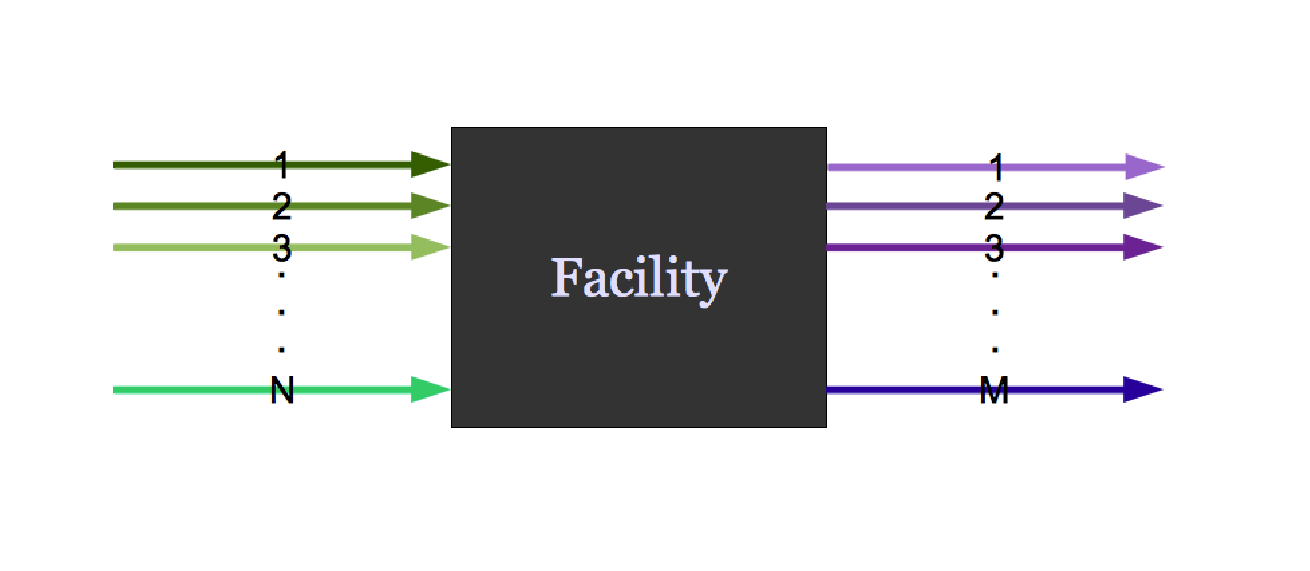
\includegraphics[height=5cm]{facility.eps}
    \end{center}
    \caption{ Regions, Institutions, Facilities, and Markets are all
    black boxes.} 
    \label{fig:sinkfacility}
  \end{figure}
\end{frame}
%---------------||||
%||||---------------
\begin{frame}[ctb!]
  \frametitle{Module Interfaces}
  \begin{figure}[htbp!]
    \begin{center}
      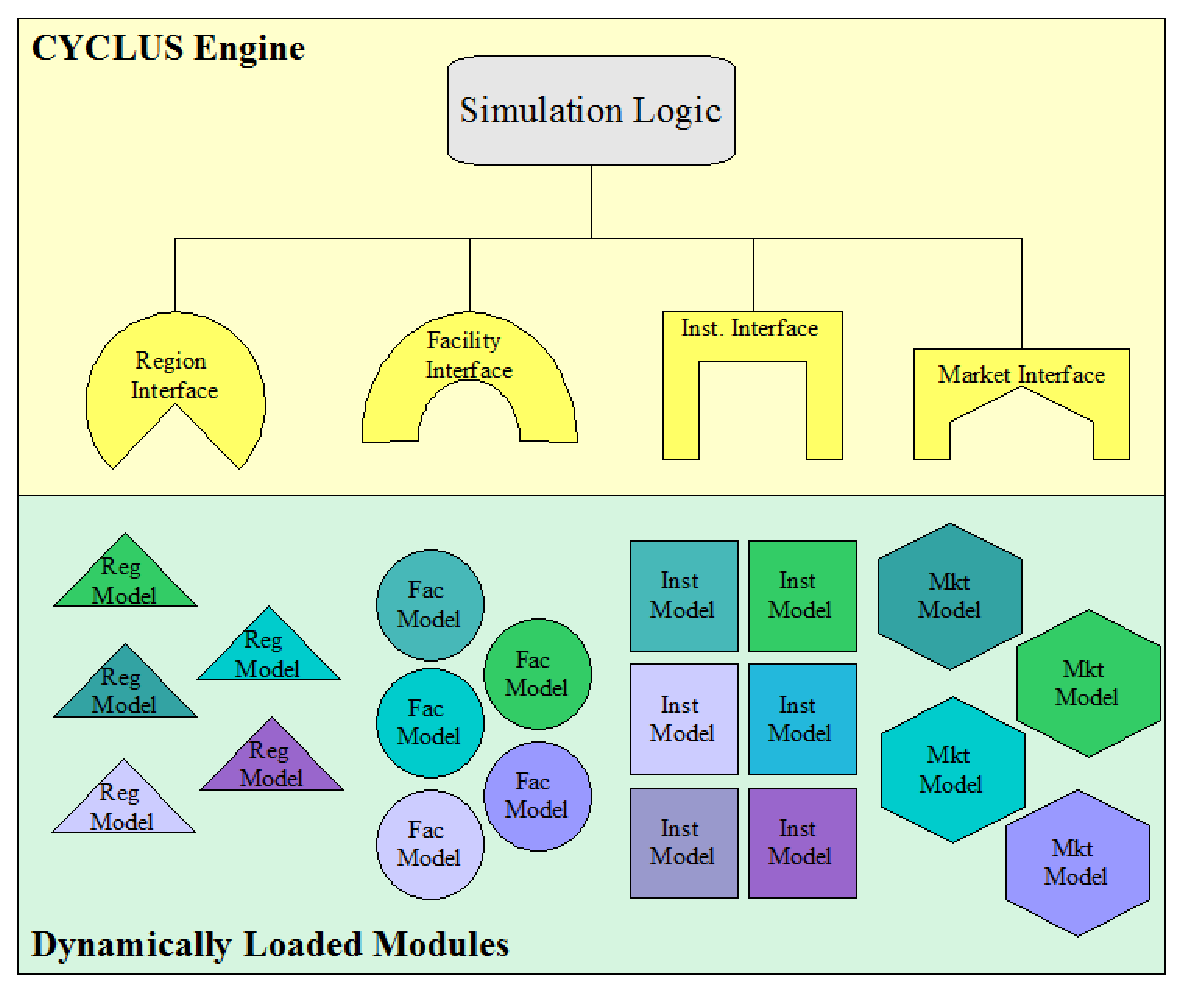
\includegraphics[height=5cm]{interfaces.eps}
    \caption{Well defined model interfaces facilitate model 
    interchange. The user may choose the model at their desired level  
    of detail.}
    \label{fig:interfaces}
    \end{center}
  \end{figure}
\end{frame}
%---------------||||

%||||---------------
\begin{frame}[ctb!]
  \frametitle{Facilities Are Black Boxes}
  \begin{figure}[htbp!]
    \begin{center}
      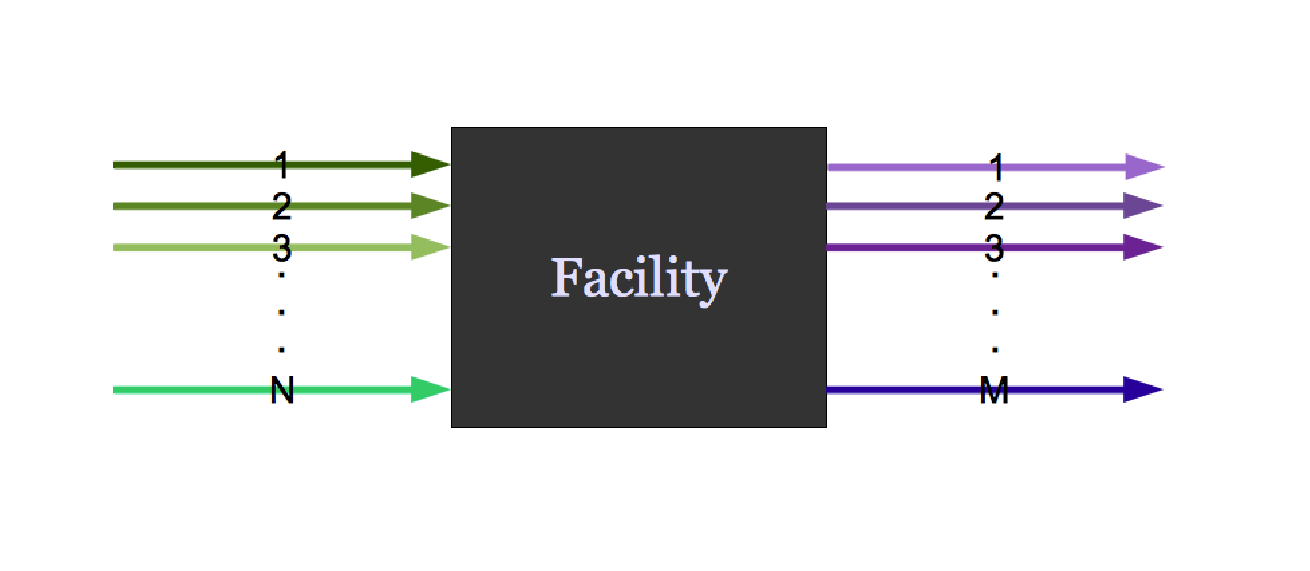
\includegraphics[height=5cm]{facility.eps}
    \end{center}
    \caption{ Each facility in the simulation makes requests and offers 
    to fill its stocks and empty its inventory respectively.  }
    \label{fig:facility}
  \end{figure}
\end{frame}
%---------------||||
%\subsubsection{Example : Market-Facility Interface}
%||||--------------
\begin{frame}[ctb!]
  \frametitle{Facilities Are Black Boxes}
  \begin{figure}[htbp!]
    \begin{center}
      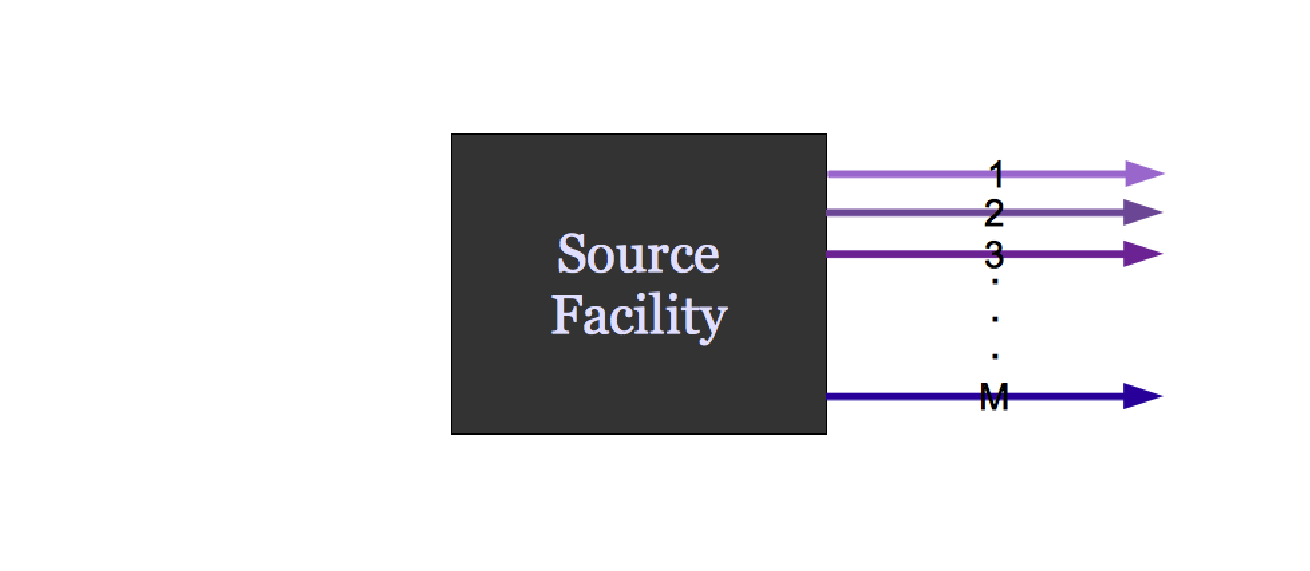
\includegraphics[height=5cm]{sourcefacility.eps}
    \end{center}
    \caption{ A facility might only make offers.} 
    \label{fig:sourcefacility}
  \end{figure}
\end{frame}
%---------------||||
%||||--------------
\begin{frame}[ctb!]
  \frametitle{Facilities Are Black Boxes}
  \begin{figure}[htbp!]
    \begin{center}
      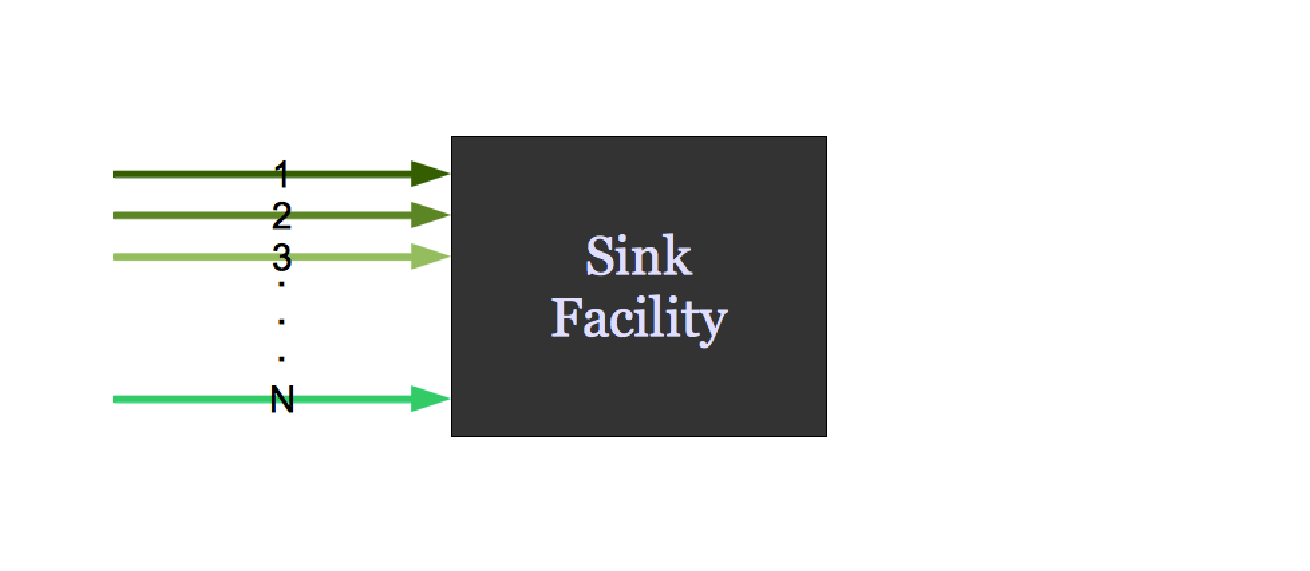
\includegraphics[height=5cm]{sinkfacility.eps}
    \end{center}
    \caption{ A facility might only make requests.} 
    \label{fig:sinkfacility}
  \end{figure}
\end{frame}
%---------------||||
%||||--------------
\begin{frame}[ctb!]
  \frametitle{Each Commodity is Associated with a Market}
  \begin{figure}[htbp!]
    \begin{center}
      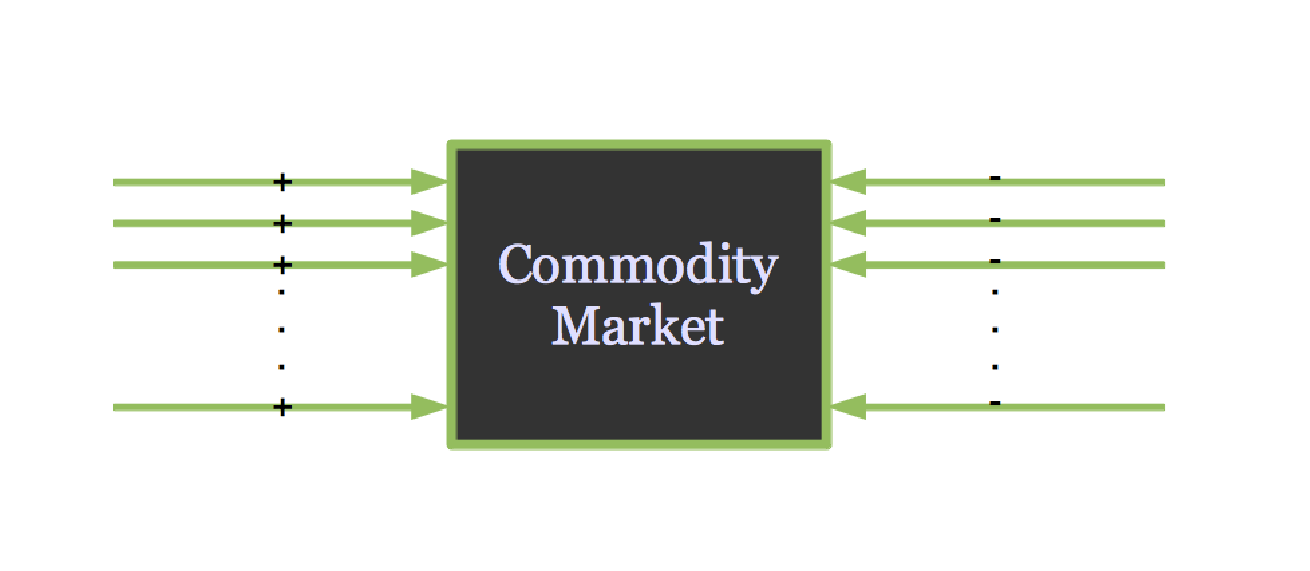
\includegraphics[height=5cm]{market.eps}
    \end{center}
    \caption{ A market receives offers and requests concerning its 
    commodity. } 
    \label{fig:market}
  \end{figure}
\end{frame}
%---------------||||
%||||--------------
\begin{frame}[ctb!]
  \frametitle{The Market Solves the Matching Problem}
  \begin{figure}[htbp!]
    \begin{center}
      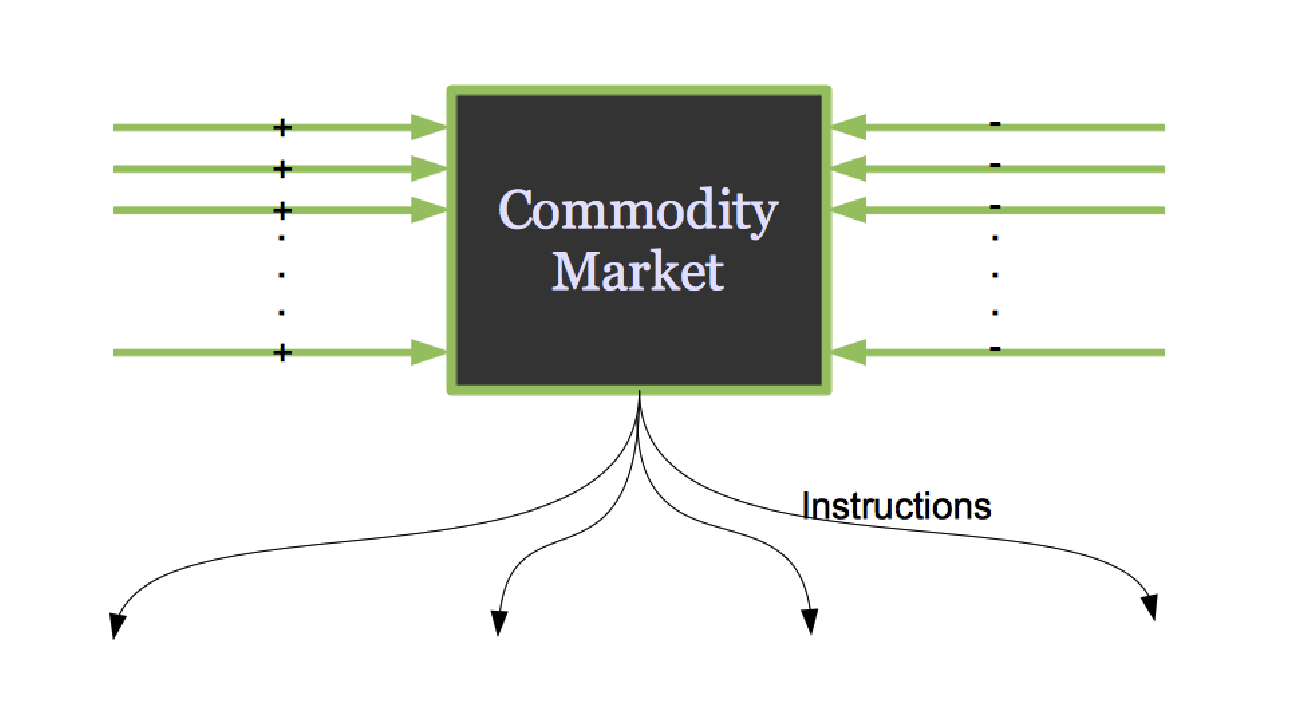
\includegraphics[height=5cm,width=8cm]{instructions.eps}
    \end{center}
    \caption{ When the Market's arbitrary algorithm solves the 
    matching problem, the Market sends instructions to the offering 
    facilities.} 
    \label{fig:instructions}
  \end{figure}
\end{frame}
%---------------||||
%||||--------------
\begin{frame}[ctb!]
  \frametitle{A Simple Example}
  \begin{figure}[htbp!]
    \begin{center}
      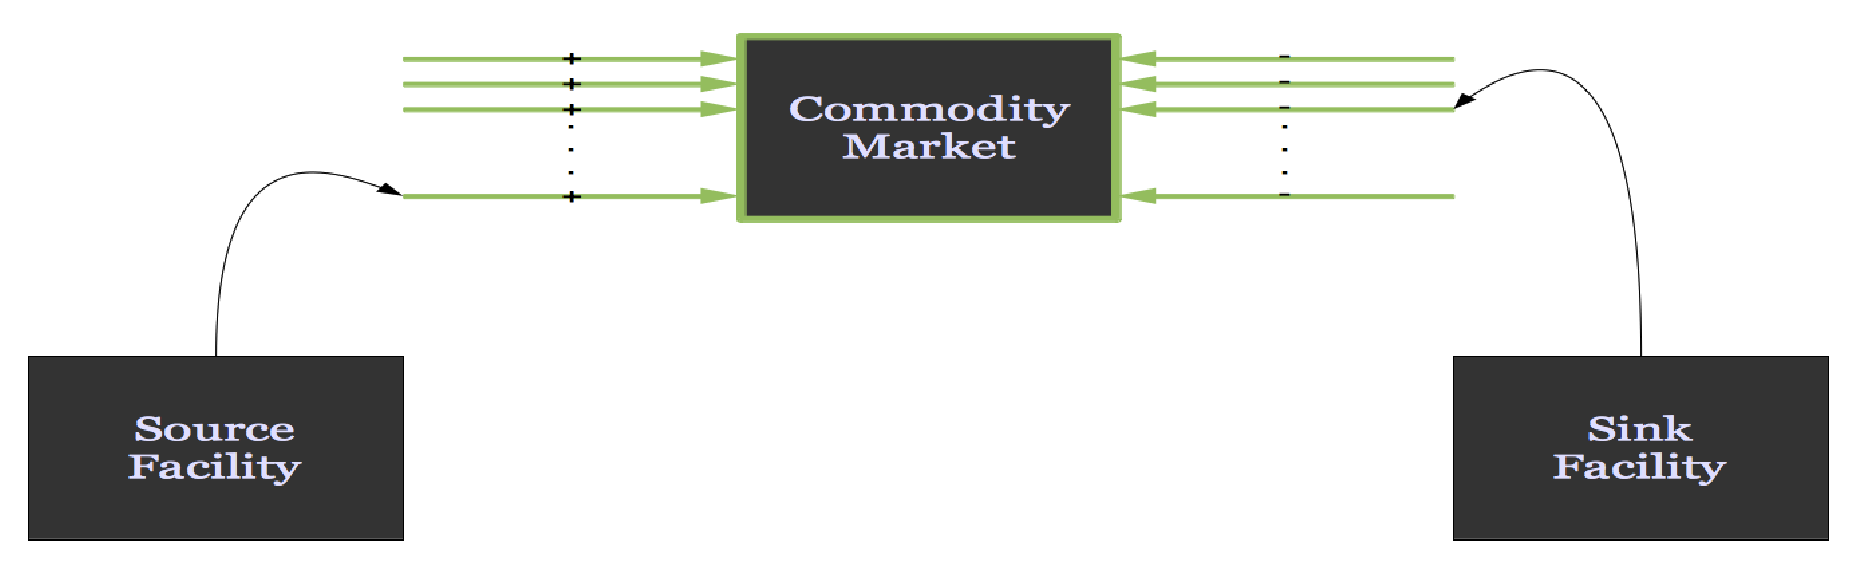
\includegraphics[height=5cm, width=8cm]{offreq.eps}
    \end{center}
    \caption{ The source sends an offer and the sink sends a request.} 
    \label{fig:offreq}
  \end{figure}
\end{frame}
%---------------||||
%||||--------------
\begin{frame}[ctb!]
  \frametitle{A Simple Example}
  \begin{figure}[htbp!]
    \begin{center}
      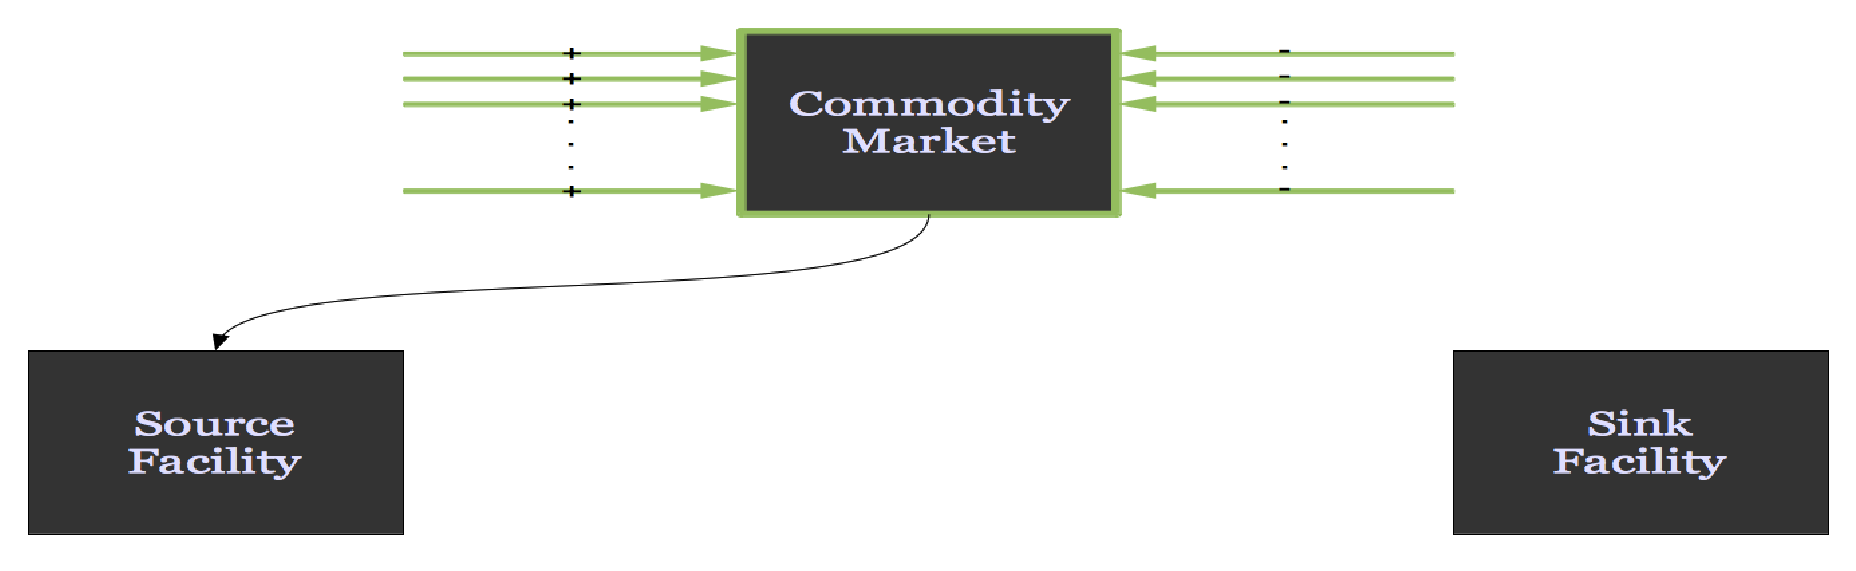
\includegraphics[height=5cm, width=8cm]{transmess.eps}
    \end{center}
    \caption{ The Market solves the problem and instructs the source 
    facility to send a certain amount to the sink facility.} 
    \label{fig:transmess}
  \end{figure}
\end{frame}
%---------------||||
%||||--------------
\begin{frame}[ctb!]
  \frametitle{A Simple Example}
  \begin{figure}[htbp!]
    \begin{center}
      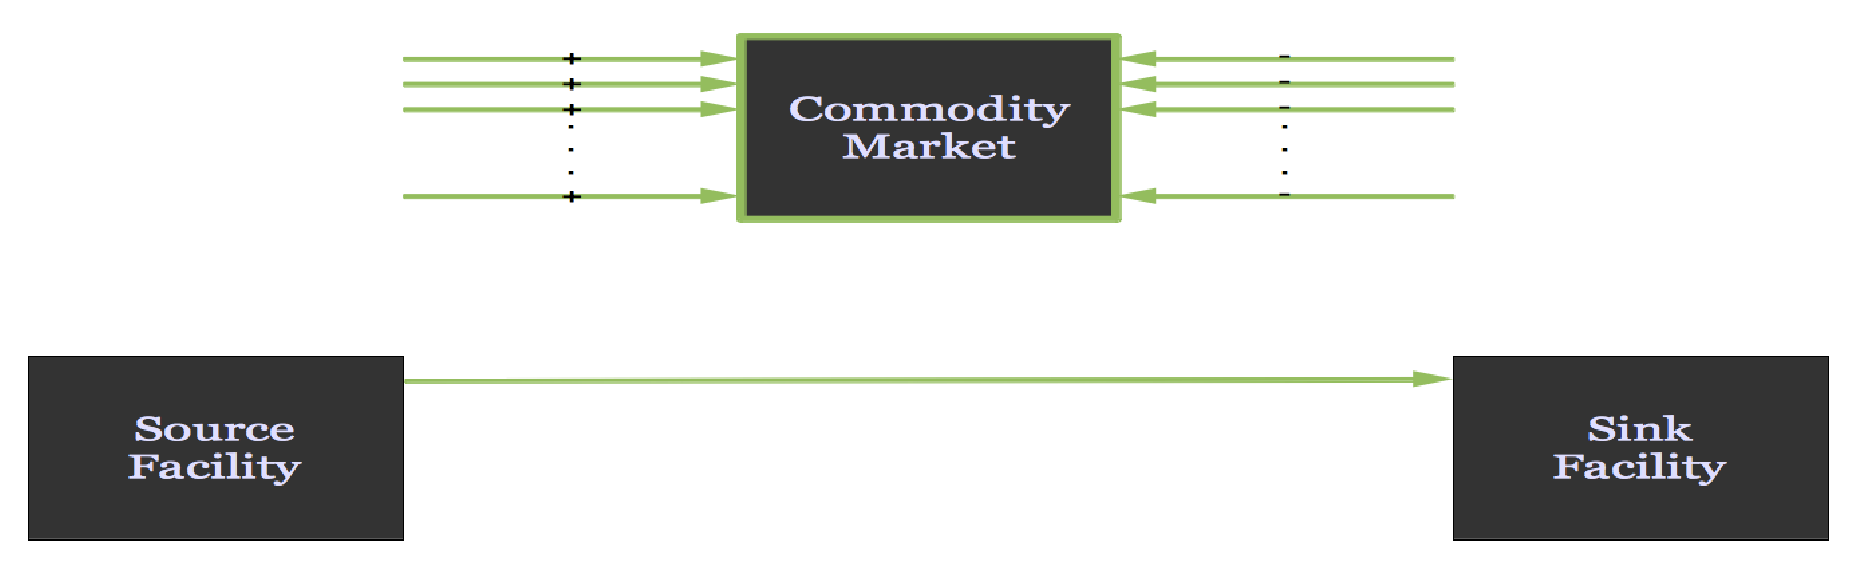
\includegraphics[height=5cm, width=8cm]{trans.eps}
    \end{center}
    \caption{ The source facility sends the material directly to the 
    sink facility.} 
    \label{fig:trans}
  \end{figure}
\end{frame}
%---------------||||
%||||---------------
\begin{frame}[ctb!]
  \frametitle{This Market Model Scales for Complex Systems}
  \begin{figure}[htbp!]
    \begin{center}
      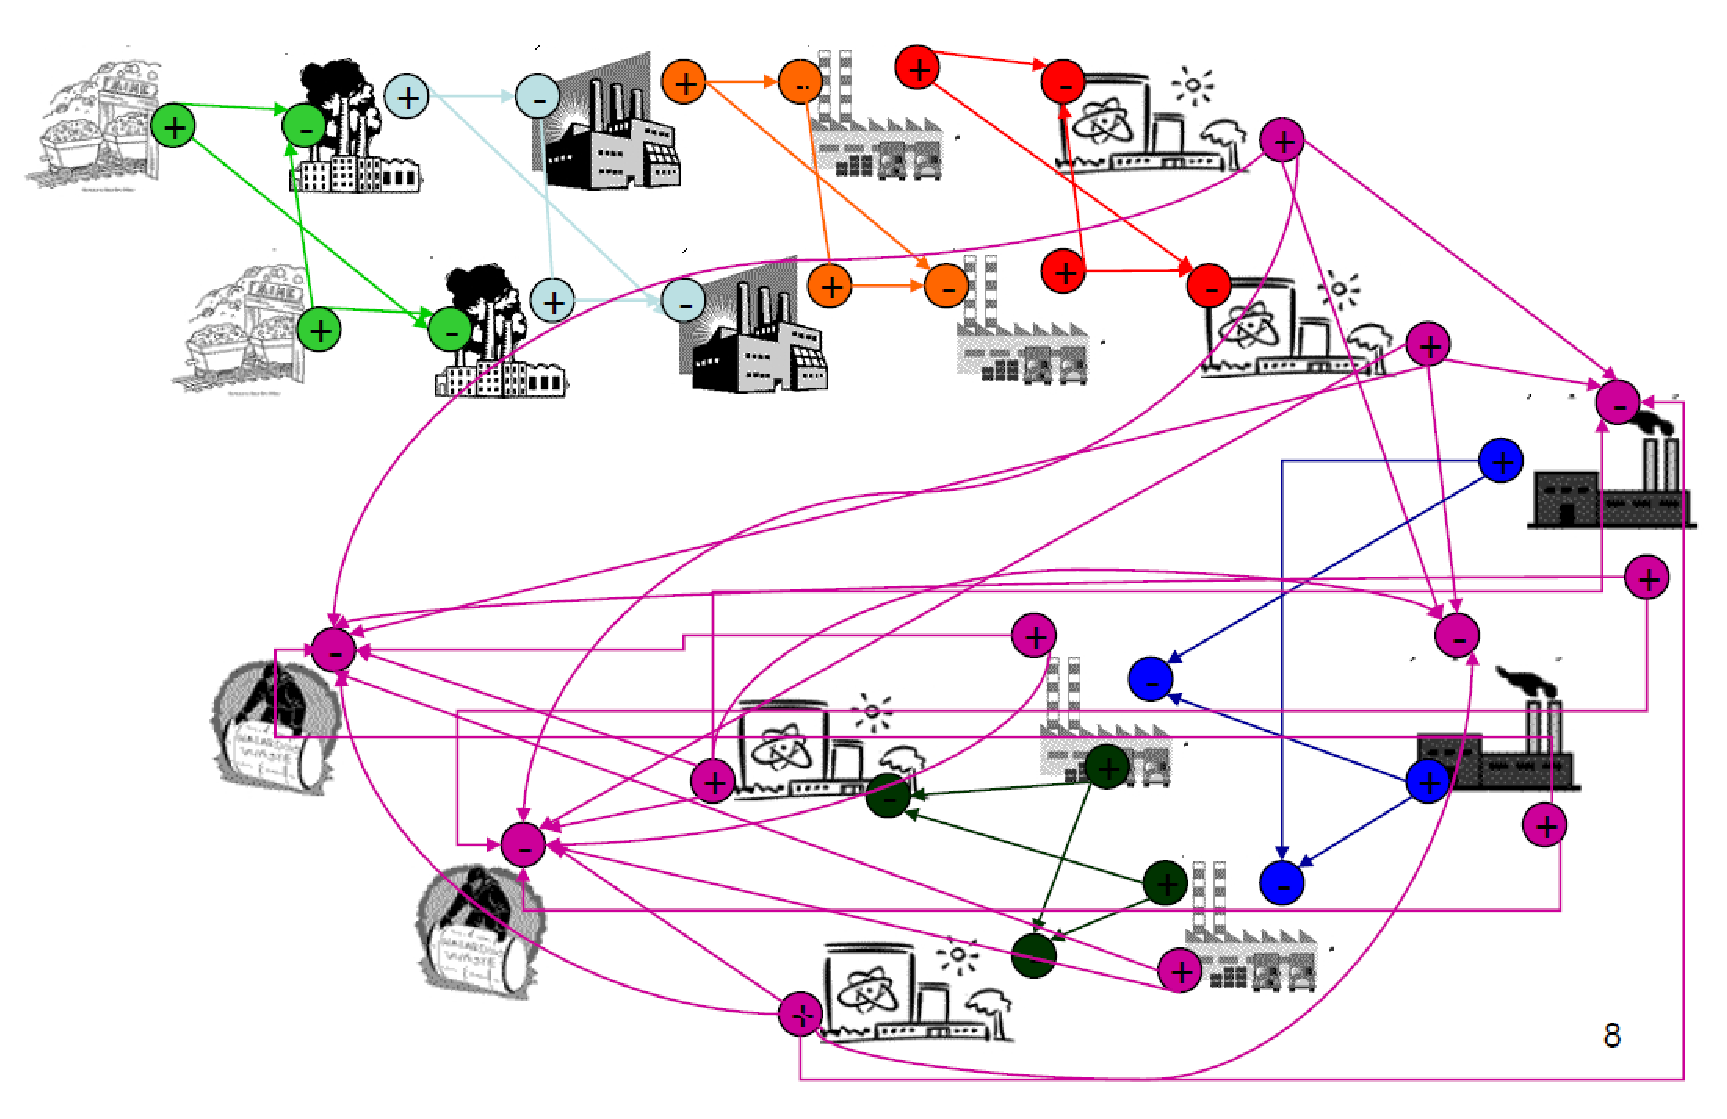
\includegraphics[height=6cm]{materials.eps}
    \end{center}
    \caption{Well designed interfaces and strict encapsulation support 
    scalability of the Market-based simulation paradigm 
    \cite{oliver_geniusv2:_2009}}
    \label{fig:materials}
  \end{figure}
\end{frame}
%---------------||||

%\subsubsection{Extensibility}
%||||---------------
\begin{frame}
  \frametitle{Dynamic Module Loading : Developer}
  With a dynamic, plug-in implementation, the simulation logic is 
  independent of the available models and models are loaded as shared 
  libraries at runtime. 

  \begin{figure}[htbp!]
    \begin{center}
      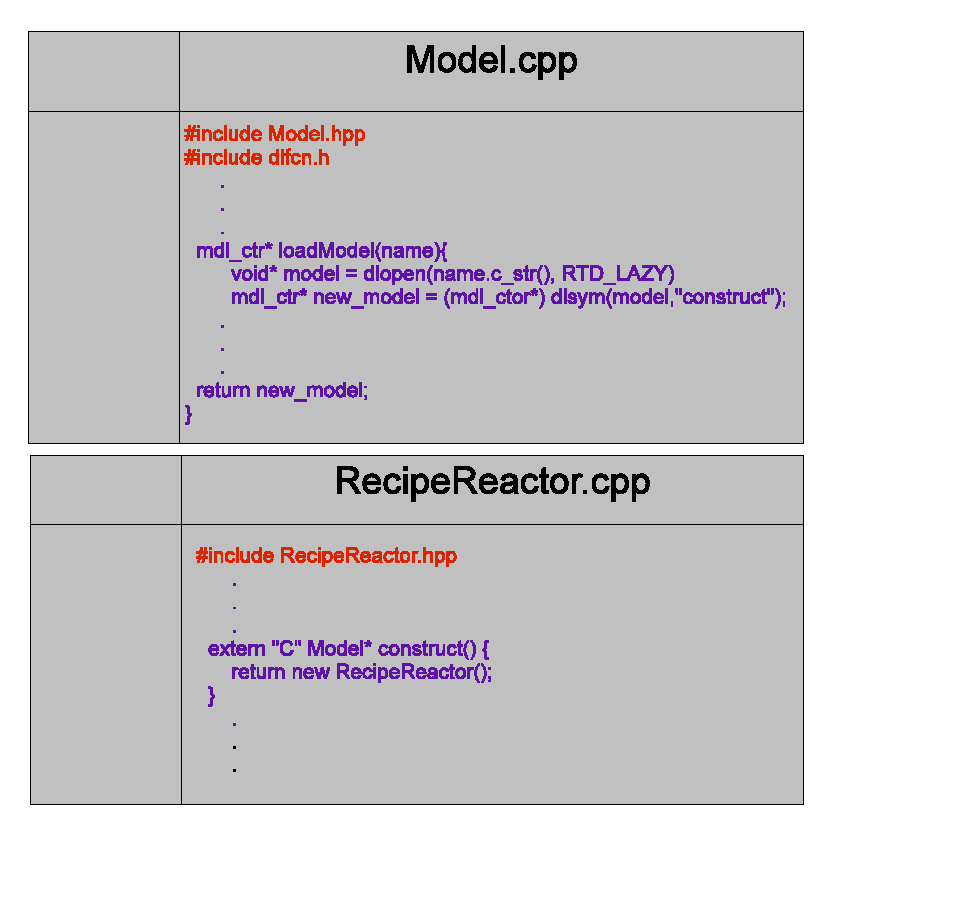
\includegraphics[height=5.5cm]{developer.eps}
    \end{center}
    \caption{Dynamic c library loading separates simulation logic from 
    knowledge of available models, supporting extensions by developers 
    with minimal lines of code.}
    \label{fig:xmlinput}
  \end{figure}

\end{frame}
%---------------||||
%||||---------------
\begin{frame}[ctb!]
  \frametitle{Dynamic Module Loading : User}
  With a dynamic, plug-in implementation, the simulation logic is 
  independent of the available models and models are loaded as shared 
  libraries at runtime. 

  \begin{figure}[htbp!]
    \begin{center}
      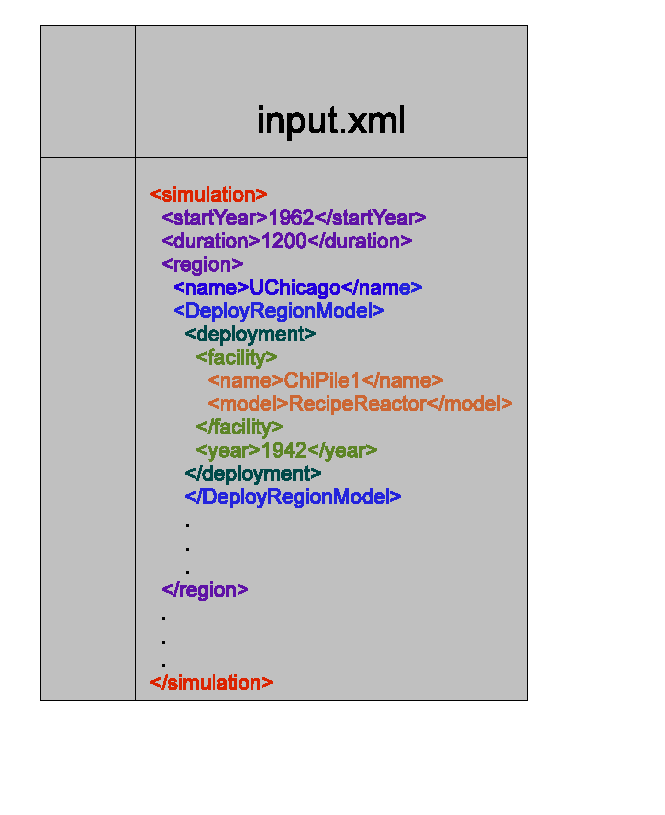
\includegraphics[height=5.5cm]{user.eps}
    \end{center}
    \caption { XML input parsing and a relaxNG schema provide 
    a simplified XML interface is available for the end
    user to define available module implementations.  }
    \label{fig:xmlinput}
  \end{figure}

\end{frame}
%---------------||||

%||||---------------
\begin{frame}[ctb!]
  \frametitle{Open Source Repository}
    This open source repository provides a centralized location for 
    documentation, developer history, and unhindered developer access.
  \begin{figure}[htbp!]
    \begin{center}
      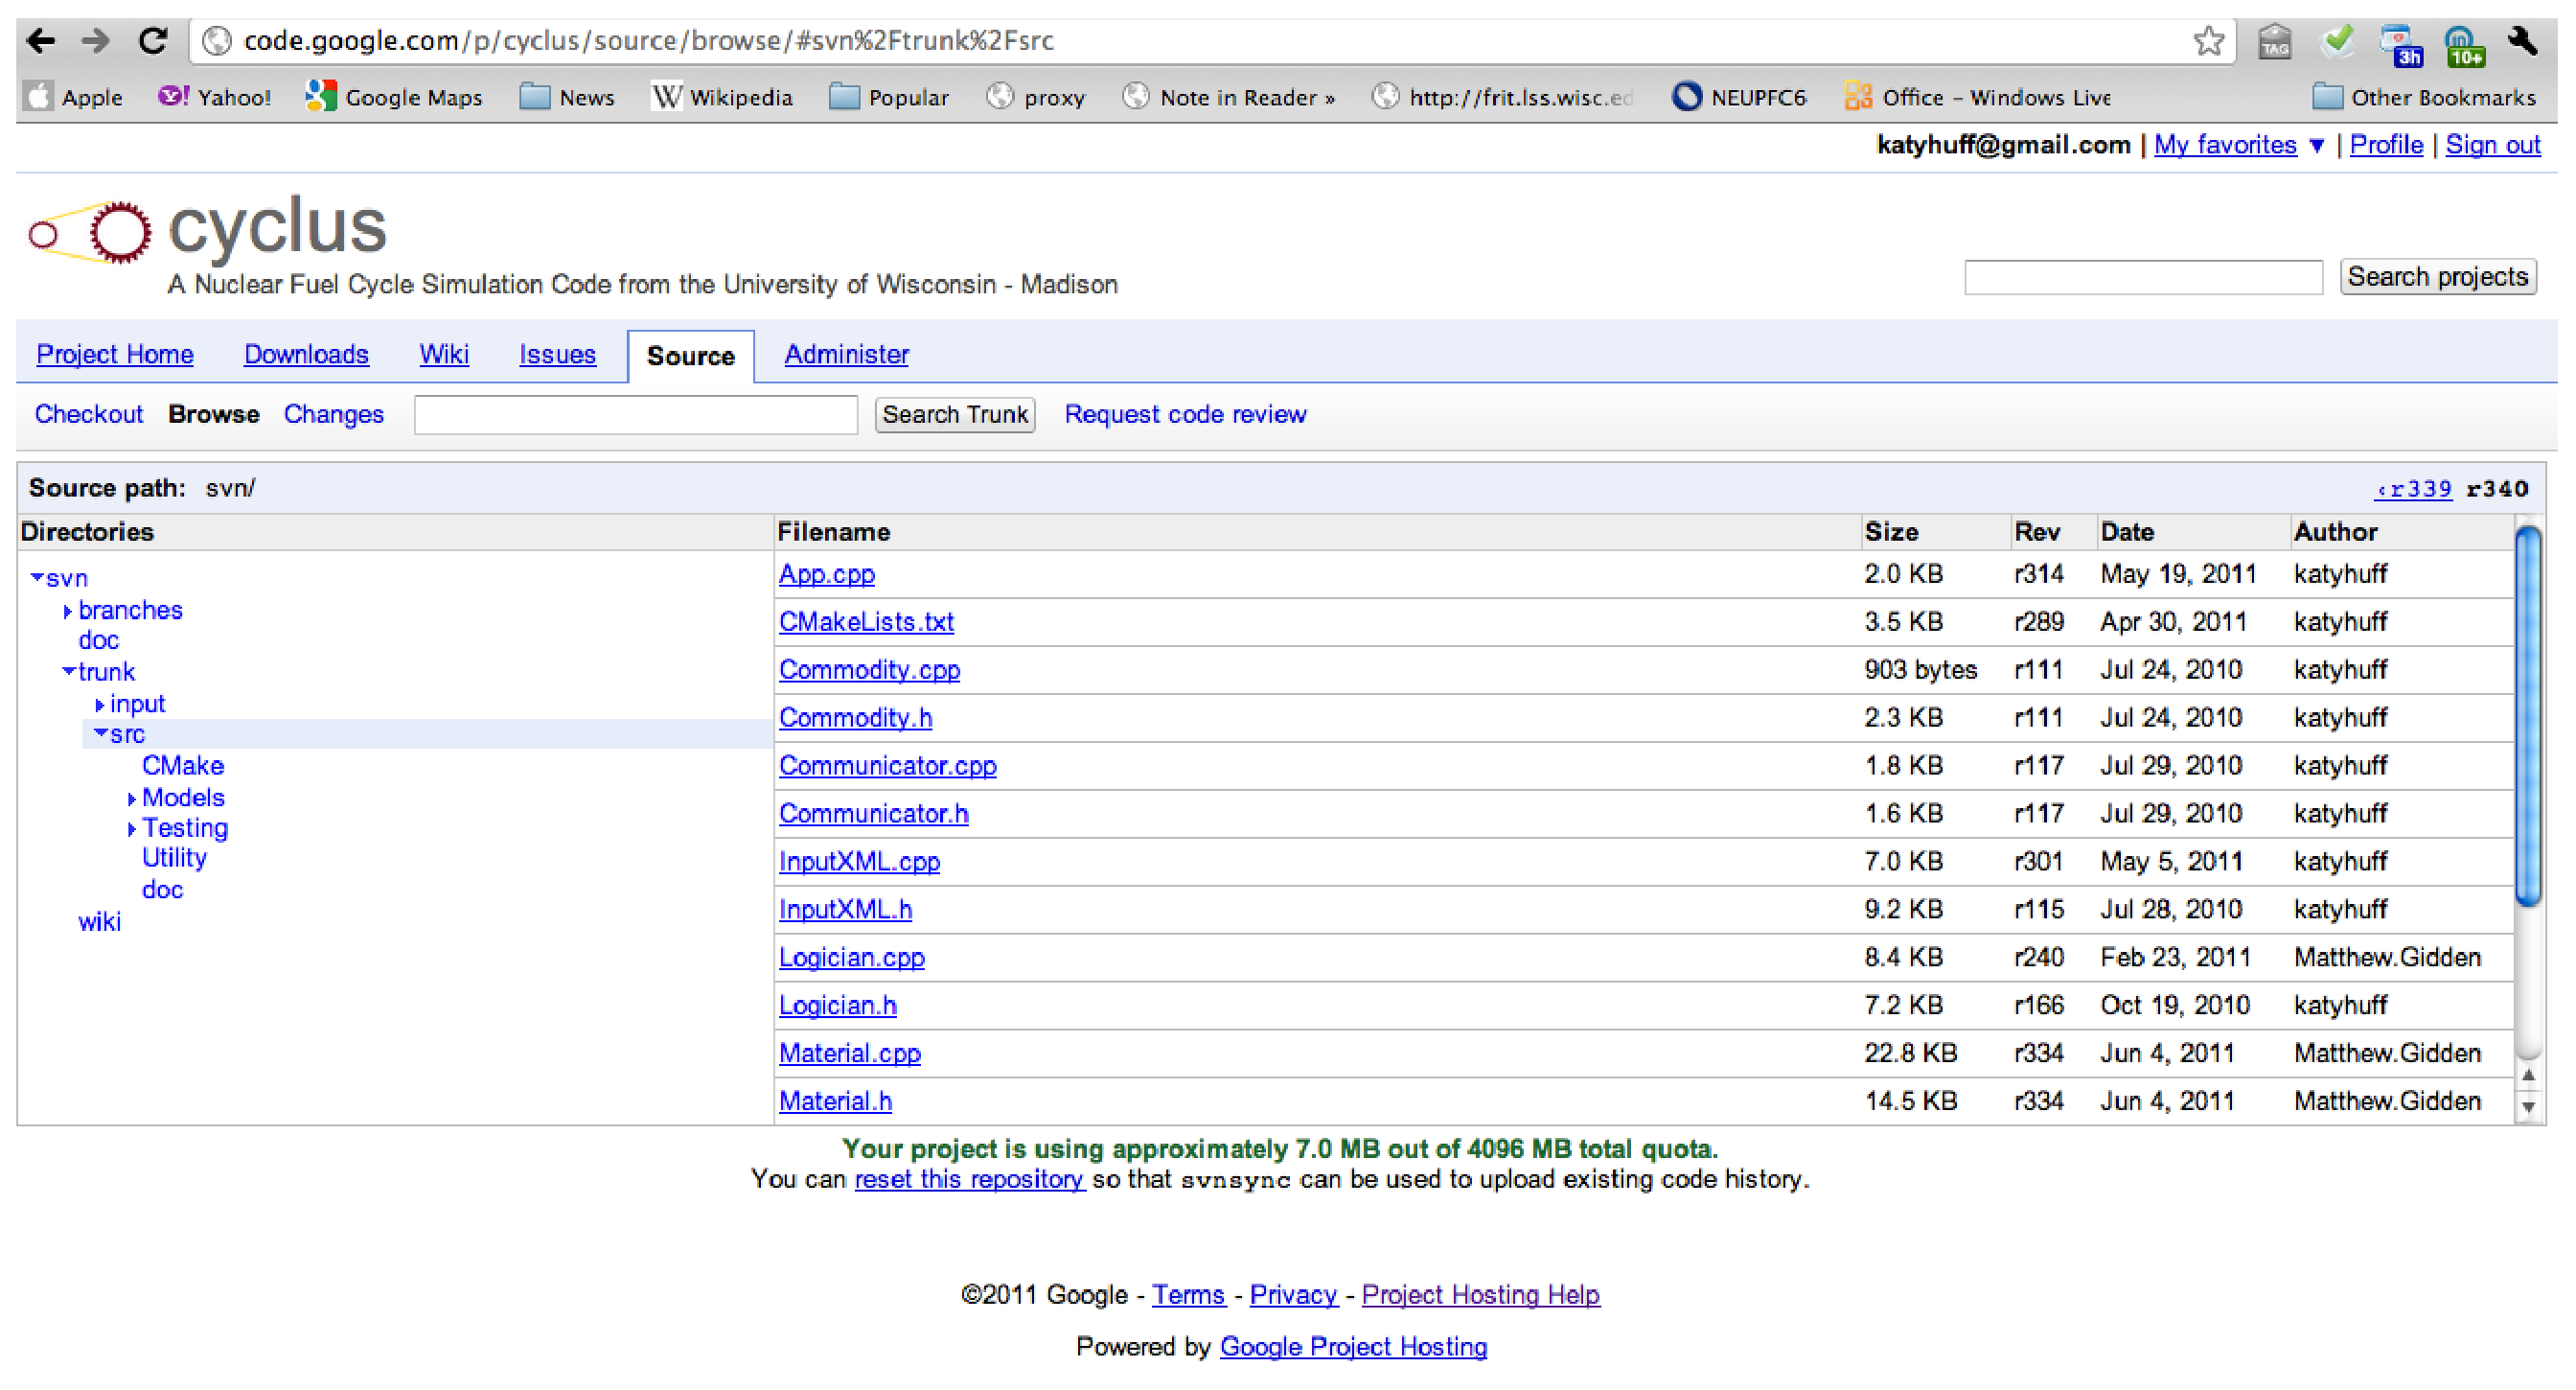
\includegraphics[height=6cm]{source.eps}
    \end{center}
    \caption{The current source code, complete revision history, and 
    documentation are made available for download and contribution 
    online. }
    \label{fig:open}
  \end{figure}
\end{frame}
%---------------||||
%||||---------------
\begin{frame}[ctb!]
  \frametitle{ `Modified Open' Source}
  \begin{figure}[hbtp!]
    \begin{center}
      
\includegraphics[height=6cm]{security.eps}
    \end{center}
    \caption{License, architecture, and development paradigm allow 
    varying levels of code sharing and data security.}
    \label{fig:security}
  \end{figure}
\end{frame}
%---------------||||
%\subsubsection{Quality Control}
%||||---------------
\begin{frame}[ctb!]
  \frametitle{Version Control}
    This open source repository employs a version control system 
     for provenance, developer access, and reproducibility of results.
  \begin{figure}[htbp!]
    \begin{center}
      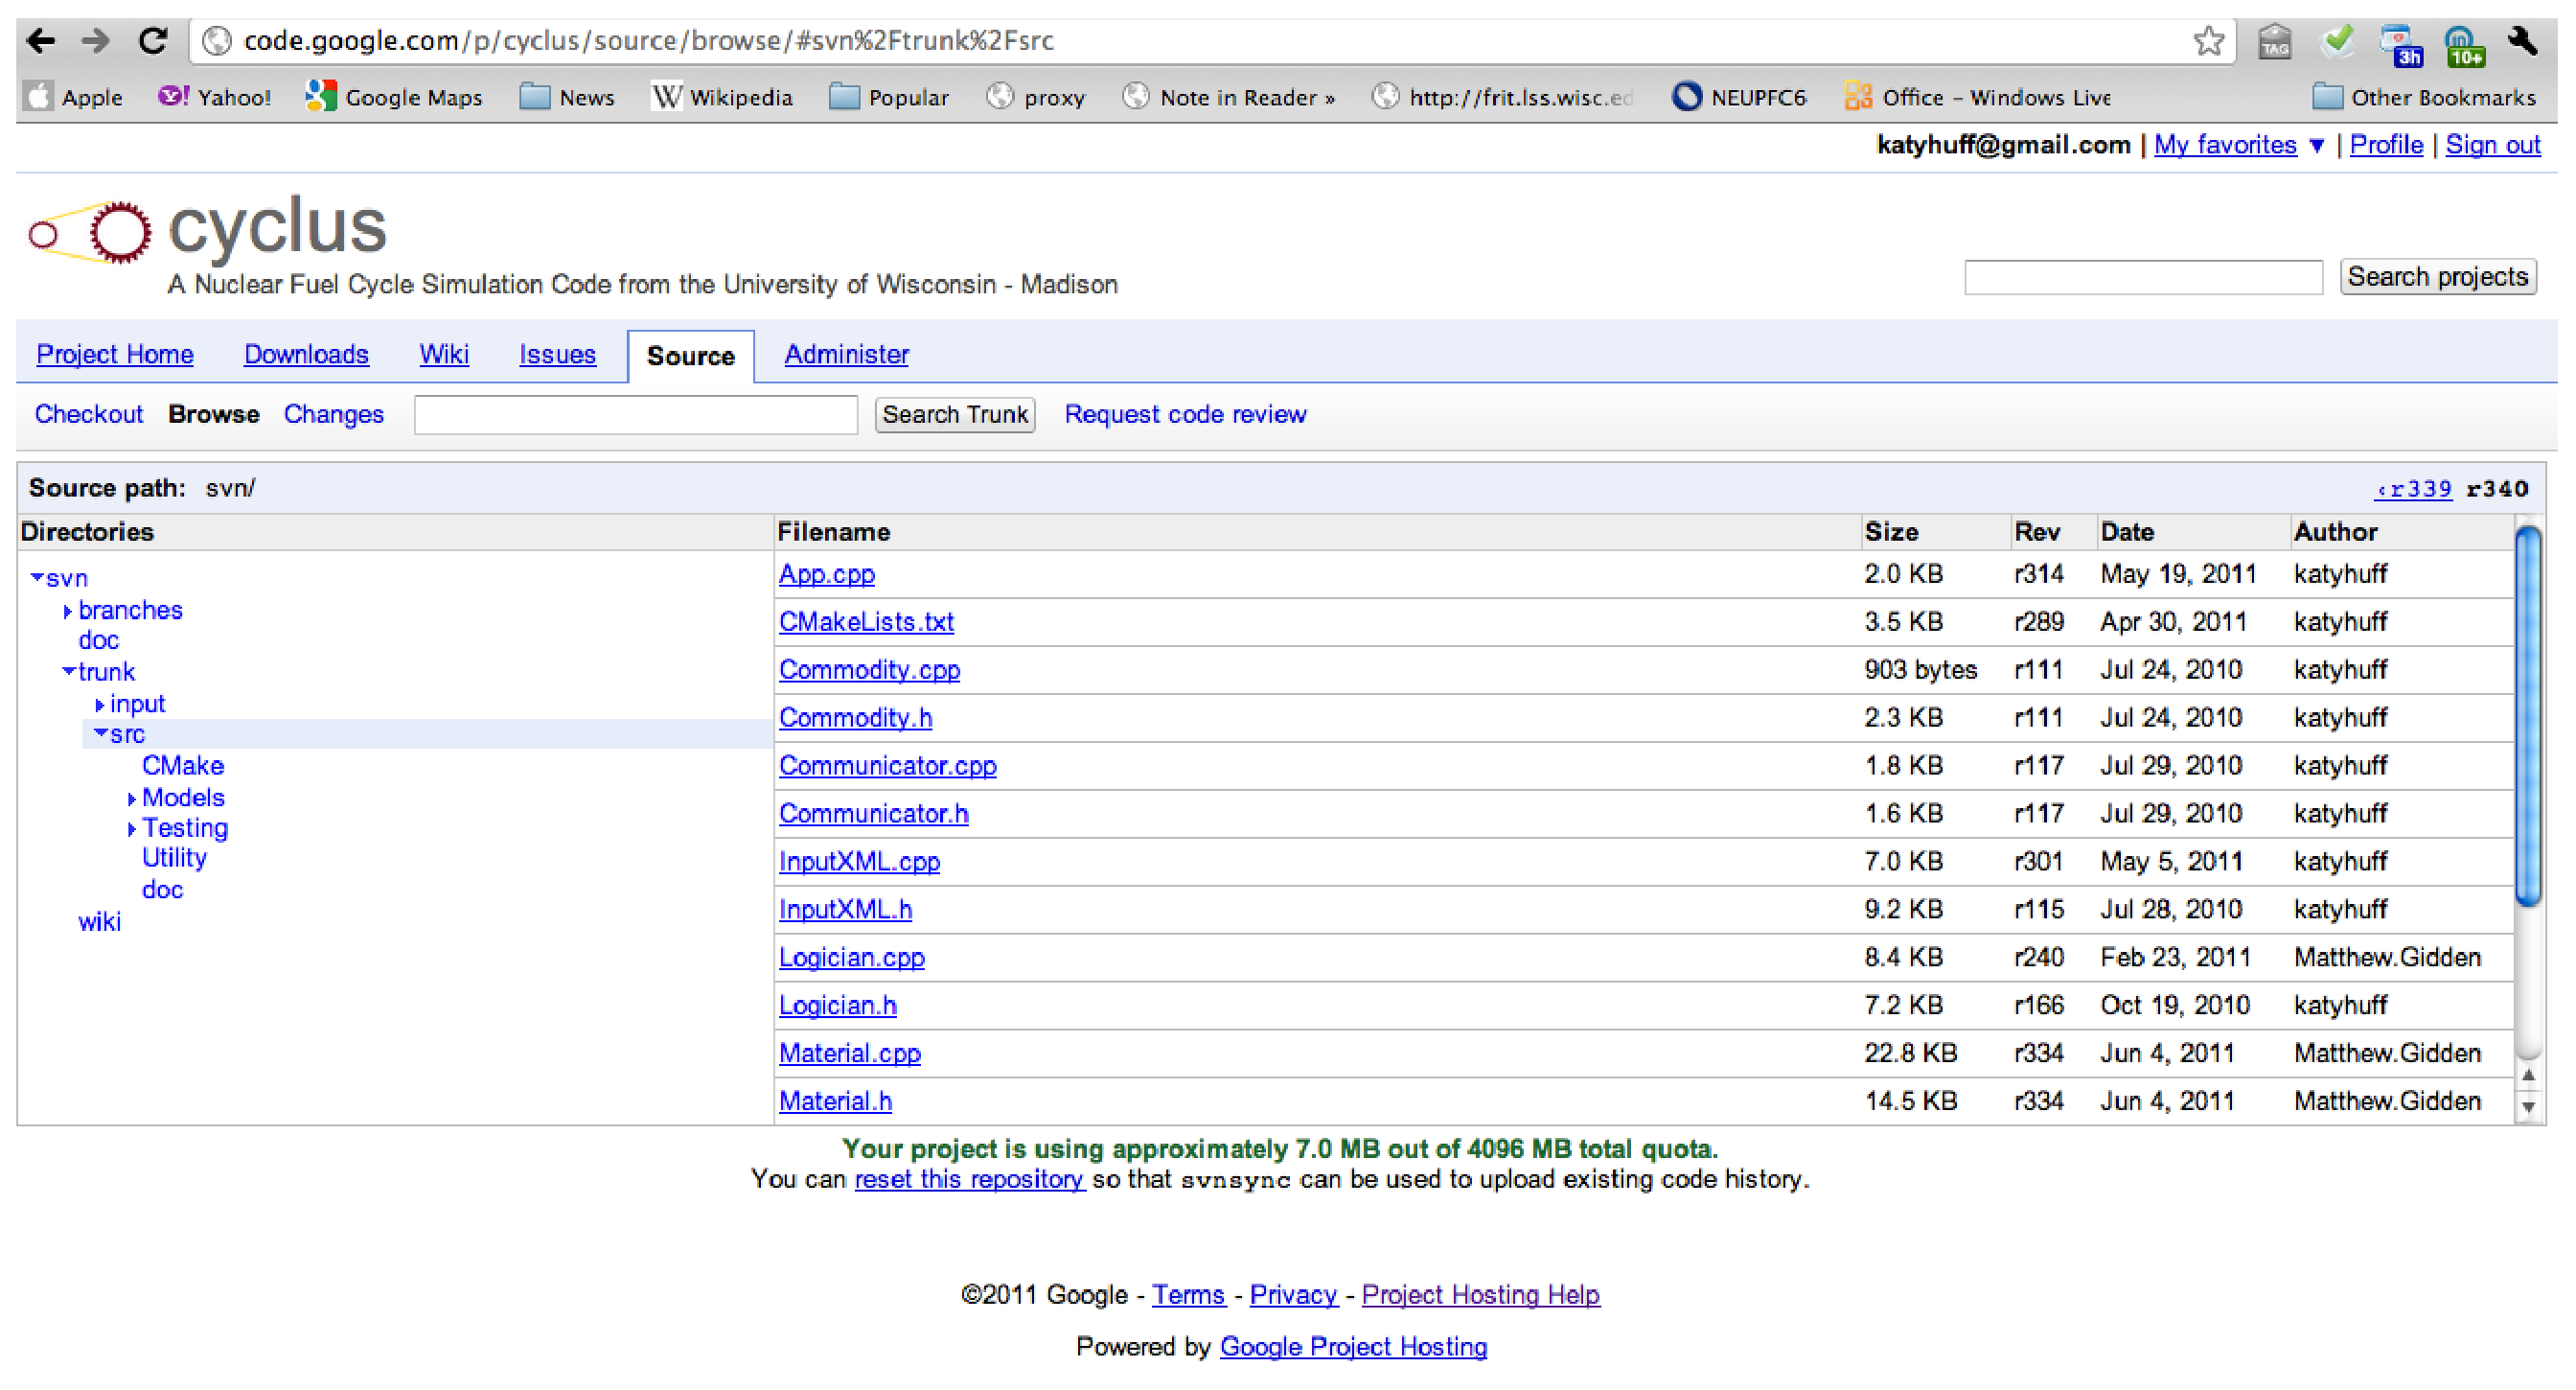
\includegraphics[height=6cm]{source.eps}
    \end{center}
    \caption{The current source code, commit messages, and complete 
    revision history is recorded and available in the repository.}
    \label{fig:source}
  \end{figure}
\end{frame}
%---------------||||
